\section{Introduction}\label{sec:intro}
What factors can explain the substantial and persistent increase in US household indebtedness over the last three decades? This question has inspired a large literature that has put forward several explanations. On the side of credit supply, the institutional framework plays a central role; \citet{CampbellHercovitz2005} emphasize the effects of the liberalization of the US home mortgage market in the early 1980s while \citet{Narajabad2012} points towards improvements in banks' risk assessment capabilities to explain an increase in credit lines available to households. On the demand side, the most influential view is arguably given by \citet{KruegerPerri2006} who interpret the expansion of US credit markets as the rational response of consumers borrowing in order to smooth out income shocks, the variance of which has risen over time. However, this view rests on the observed increase in cross-sectional income variation being largely due to a rise in the variance of transitory idiosyncratic shocks, an interpretation that has been called into question by several authors. As an example, \citet{KopczukSaezSong2010} find that the rise in income inequality was almost entirely driven by increases in permanent earnings inequality, with no mitigating effect of mobility across income groups that decreased at the same time as earnings inequality increased. In the same vein, \citet{DHPRV2013} use a confidential panel of tax returns from the IRS to show that all of the rise in the variance of male labour earnings between 1987 and 2009 can be attributed to a rise in the variance of the persistent part of income. In light of these difficulties, the present work aims to examine an additional mechanism that could drive household credit demand -- consumption habits. In this regard, this work bears some resemblance to the prominent \citet{Rajan2011} hypothesis that the foundations for the financial crisis of 2007/08 were laid by a credit expansion that mostly benefited low-income households. This also relates to more heterodox, post-Keynesian and Marxist explanations of rising household indebtedness that emphasize the role of debt as a substitute for stagnating or declining real wages in the middle and lower percentiles of the income distribution (see, for example, \citealp{BarbaPivetti2009}), a mechanism of course that would require households to be -- at least for some time -- oblivious towards the realities of the path of their income stream. Often, behavioural explanations such as conspicuous consumption or household optimization based on a relative income hypothesis are invoked, examples include \citet{BertrandMorse2012}, who find empirical support for the hypothesis that consumption of lower income households is influenced by consumption of high income households, and \citet{vanTreeck2012}, who presents some calculations based on Duesenberry's (1940) relative income hypothesis. Here, we try to frame this argument in terms of an arguably more standard economic model: a life-cycle model with fully optimizing rational households that derive utility from current and past consumption, while facing an uncertain income stream that they learn about over the course of their working life. The basis for the present analysis is a model introduced by \citet{Guvenen2007}, in which the income process consists of a permanent stochastic AR(1)-component, as is standard in most of the literature, and an additional deterministic term, that is different across workers and that they have to learn about in order to make precise forecasts of their lifetime income. This uncertainty, coupled with the time-inseparability of consumption introduced by habit formation, can under certain circumstances lead to an increase in the indebtedness even of households with permanently low incomes. \\
The remainder of this paper is structured as follows: Section (\ref{sec:sf}) presents some stylized facts on the developments of the US income and wealth distribution that motivate this work. Section (\ref{sec:model}) lays out the model and gives analytical results for a stripped down version of the model that shed light on the mechanisms through which habit formation can generate higher indebtedness. Section (\ref{sec:qr}) presents the results of a quantitative evaluation of the model that is informed by data from the CEX and the SCF. Section (\ref{sec:ext}) extends the model to include a labour supply decision and gives results for different assumptions on prior uncertainty, learning behaviour and the specification of the habit formation process. Section (\ref{sec:disc}) discusses the success of different versions of the model in replicating observed data. 


\pagebreak
\section{Stylized Facts}\label{sec:sf}
The widening inequality in the U.S. income distribution is a well documented feature of the data during at least the last three decades. Numerous studies have examined the secular rise in top incomes (\citealp{PikettySaez2003}) and the flattening path of middle and lower incomes (\citealp{AutorKatzKearney2005}) and put forward explanations such as changes in relative demand and supply for different skill levels, the decline of union power, increases in international trade and competition (\citealp{Ma2013}) and the fall in the real value of the federal minimum wage\footnote{Some doubts on the magnitude and timing of the rising inequality are raised by \citet{Gordon2009}.}. While the exact timing and magnitude of the rise in inequality may differ slightly from one data source to the other and depending on the exact definition of income employed, its existence can be regarded as a consensus in the literature. Figure (\ref{fig:inc_ineq}) is taken from Attanasio, Hurst and Pistaferri (2012) and shows the evolution of income inequality at different points of the income distribution from 1980 to 2010 based on PSID data. The rise in overall inequality is apparent and can be seen to be mostly driven by a surge in top incomes (even though, as the authors note, PSID data undersamples very rich households and thus most likely understates the rise in top incomes). 
\begin{figure}[ht]
	\centering
		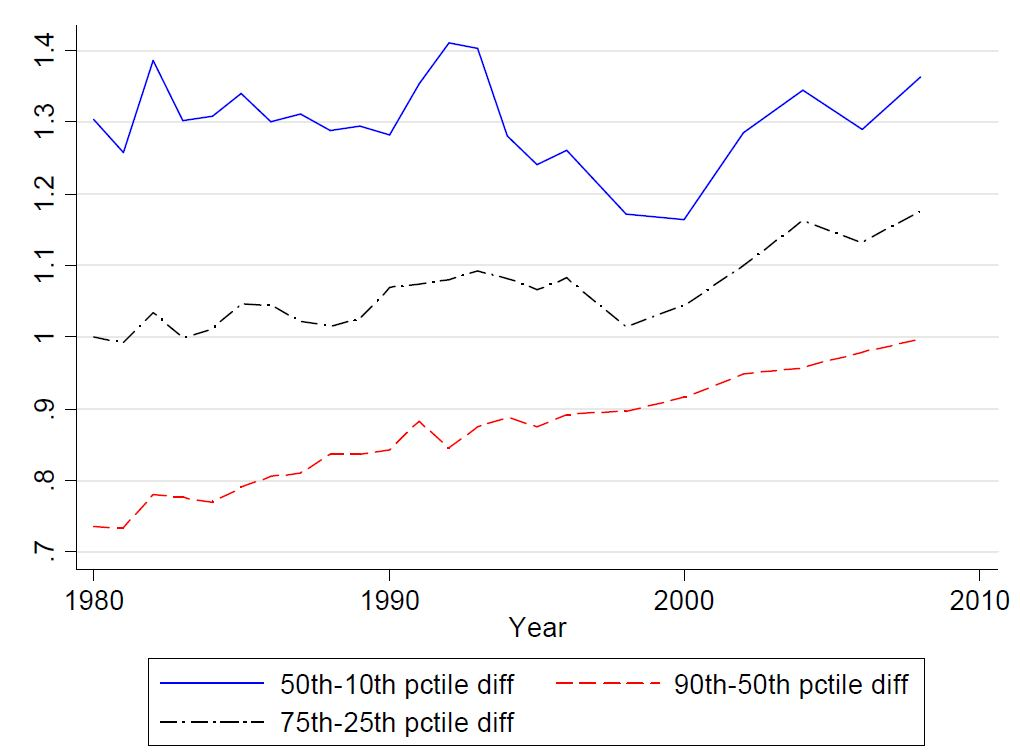
\includegraphics[width=0.85\textwidth]{inc_ineq_attanasio2012.JPG}
		\caption{Income inequality for three income differentials, 1980-2010, PSID data}
	\label{fig:inc_ineq}
\end{figure}
There exists less consensus about the evolution of consumption inequality over the same period. While early prominent studies such as \citet{KruegerPerri2006} used CEX data to argue that there has been virtually no increase in consumption inequality and built theoretical models that could account for this puzzle, more recently other authors have found a larger increase in consumption inequality using different data sources that arguably suffer from less measurement error than the aggregate CEX data. \citet{HeathcotePerriViolante2010} use CEX spending data to document a very modest increase in consumption inequality, while \citet{AguiarBils2011} use the difference between income and spending in CEX data to document a rise in consumption inequality that is almost as large as the rise in income inequality and \citet{AHP2013} argue that, looking at some of the more precisely measured items in the CEX, one finds that consumption inequality has indeed tracked income inequality. For the purpose of this paper, we will use aggregate spending data from the CEX and thus assume that consumption inequality has not risen to the same extent as income inequality while keeping in mind that this is not a foregone conclusion. We will return to this point in the last chapter. \\
Another well documented feature of the data is the rise in debt holdings of the private sector. As with the rise in income inequality, this development has been widely noted and discussed with numerous explanations put forward, including changes in the regulatory framework and banking technology that widened credit supply. Most relevant to this work is the demand side argument of \citet{KruegerPerri2006}, who explain the rise in indebtedness with a limited commitment model in which the variance of the transitory component rises and hence more insurance is required, and, indeed, optimal from a welfare perspective. However, as \citet{Cordoba2008} points out, their model produces to empirically unappealing results: for one, wealth holdings are not concentrated at the top of the distribution, and second, the model predicts a large fraction of agents in the economy with negative wealth holdings, when their number really is close to zero in the data. Furthermore, their argument is weakened by a number of studies that find changes in the variance of the permanent component of income shocks to be the driving force behind the rise in income inequality. This is hard to reconcile with the fact that individuals at the lower end of the income distribution are those that increased their debt holdings the most. Figure (\ref{fig:chg_debt_scf}) shows the changes in debt holdings for various debt categories calculated from SCF data for 1989 to 2007. 

\begin{figure}[ht]
	\centering
		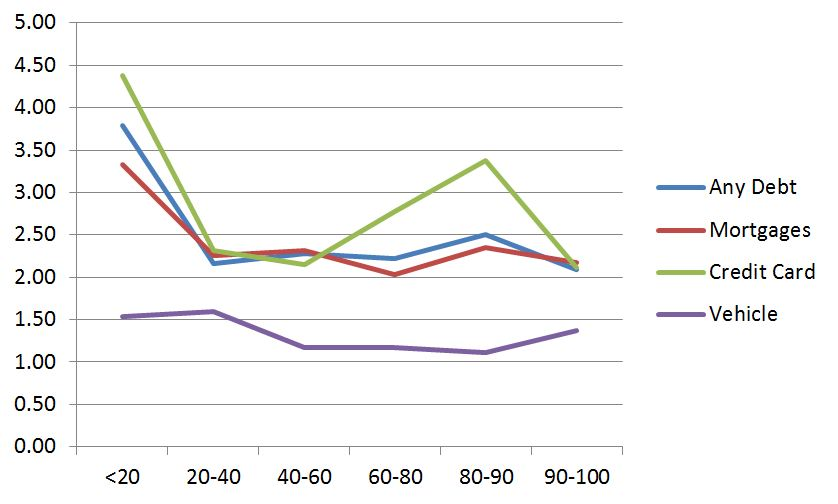
\includegraphics[width=0.85\textwidth]{chg_debt_scf}
		\caption{Changes in debt holding by income percentile, 1989-2007, Source: SCF}
	\label{fig:chg_debt_scf}
\end{figure}

While the large rise in indebtedness for the lowest income group is an artefact of business owners with failed businesses in the data, it is interesting to note that the rise in overall debt has been at least as large for the 20th to 60th percentile as for the highest income percentile. This comes as a surprise if one takes into account the higher income growth rates for individuals in higher income quintile since the early 1980s. Assuming that the dispersion in incomes is mostly driven by an increase in dispersion in the permanent component of income (as suggested by, among others, Kopczuk et al., 2010), a standard life-cycle model would suggest that while high income households should borrow against their higher future income, low income households wouldn't have an incentive to borrow when wages are stagnant. Furthermore, note that the data is not scaled by income, so that debt holdings relative to income have increased a lot more for lower income households, given that their income growth rates over the same period have been lower than those of higher income households. Indeed, \citet{BarbaPivetti2009} find that instalment loans and credit card debt amount to 59\% of disposable income for households in the lowest income quintile of the 2004 SCF, while they amount to only 11\% for the highest quintile. \\
One adjustment margin for households that could explain a decoupling of income and consumption inequality at least over short to medium frequencies is obviously saving. \citet{SaezZucman2014} find that the share of wealth holdings of the bottom 90\% of the wealth distribution has fallen from 35\% in the mid 1980s to 23\% in 2012, citing low growth of middle-class income, financial deregulation leading to predatory lending and behavioural biases in savings decisions as possible explanation. This paper can be seen as an attempt to investigate to what extent imperfect information of agents can account for the observed change in the wealth distribution.  

\begin{itemize}
\item Increase in the dispersion of wealth holdings that tracked or exceeded the rise in income inequality
\item Decreasing aggregate savings rate
\item Prevailing misperceptions about future economic situation (Moore 2003)
\end{itemize}

\pagebreak
\section{The Model}\label{sec:model}
The modelling approach draws heavily on the approach in \citet{Guvenen2007} and mostly follows the notation therein. As in Guvenen's work, consumers maximize utility from consumption over the life-cycle while facing an uncertain income stream that consists of a common, known component capturing experience effects, an unknown, individual specific linear term that agents have to learn about, an AR(1) component and a purely transitory shock. The important departure in this work is that consumers also build a stock of habit that enters the utility function multiplicatively, as is standard in the literature to avoid numerical problems with CRRA utility functions (for a discussion, see \citet{Carroll2000}). 
Consumers maximize
\begin{align}
E_0 &\left[ \sum_{t=0}^{T} \beta^{t} \frac{\left( c_{t}^{1-\gamma} \left( \frac{c_{t}}{h_{t}} \right)^{\gamma} \right)^{1-\sigma}}{1-\sigma} \right] \label{eq:maxprob} \\
\intertext{s.t. } &h_{t+1} = (1-\lambda)h_t + \lambda c_t \label{eq:habits} \\
									&a_{t+1} = (1+r)a_t + y_t - c_t \label{eq:bc} \\
									&y_{t}^i = g(\theta^0, X_t^i) + f(\theta^i, X_t^i) + z_t^i + \epsilon_t^i \label{eq:incproc} \\
  								&a_{t+1} \geq \underline{a} \label{eq:borrcons} 
\end{align}
where $c_t$ is consumption in period $t$, $h_t$ is the habit stock accumulated up to period $t$, $a_t$ are asset holdings subject to a borrowing constraint $\underline{a}$ -- the specification of which will not be straightforward in this model and requires some further discussion -- and $y_t^i$ is individual income, that can further be broken down into several parts: 
\begin{equation*}
y_{t}^i = g(\theta^0, X_t^i) + f(\theta^i, X_t^i) + z_t^i + \epsilon_t^i 
\end{equation*}
where $g(\theta^0, X_t^i)$ captures age effects and individual specific characteristics such as education, $z_t^i$ is an autoregressive process of order one, and $f(\cdot)$ is an individual specific function that plays the decisive role in introducing heterogeneity and learning in the model.
\begin{align*}
f(\theta^i, X_t^i) &= \alpha^i + \beta^i t \\
z_t^i &= \rho z_{t-1}^i + \eta_t^i \\
\theta^i &\sim N \left[ \begin{pmatrix} 0 \\ 0 \end{pmatrix}, \begin{pmatrix} \sigma_{\alpha}^2 & \sigma_{\alpha \beta} \\ \sigma_{\alpha \beta} & \sigma_{\beta}^2 \end{pmatrix} \right]
\end{align*}
The parameters $\alpha$ and $\beta$ are randomly distributed over the population and govern the evolution of lifetime income over time. Furthermore, they are unknown to individuals upon entering the labor market, meaning that in order to calculate an expected lifetime income to base consumption (and thus, implicitly, habit) choices on, consumers in the model have to hold beliefs over the values of their individual parameters. Here again we follow Guvenen in assuming that these beliefs are updated in a Bayesian fashion, which means beliefs are updated by solving a Kalman filtering problem. \\
Denoting by $S^i_{t+1}$ the vector of parameters $\alpha^i$, $\beta^i$ and $z^i_{t+1}$ and by $F$ the coefficient vector in the state space representation, we can derive an optimal forecast based of Bayesian updating for the evolution of the individuals belief about the evolution of $S^i_t$ as 
\begin{align}
\hat{S}^i_{t|t} &= \hat{S}^i_{t|t-1} + P_{t|t-1} H_t [H_t' P_{t|t-1} H_t + R]^{-1}(y_t^i - H_t' \hat{S}^i_{t|t-1}) \label{eq:KFS} \\
\hat{S}^i_{t+1|t} &= F \hat{S}^i_{t|t} \label{eq:TES}
\end{align}
where $P_{t|t}$ is the variance-covariance matrix of $\hat{S}^i_{t|t}$ and $R$ is the variance of the transitory shock. A similar expression can be derived for the evolution of $P_{t+1|t}$:
\begin{align}
P_{t|t} &= P_{t|t-1} - P_{t|t-1} H_t [ H_t' P_{t|t-1} H_t + R]^{-1} H_t' P_{t|t-1} \label{eq:KFP} \\
P_{t+1|t} &= F P_{t|t} F' + Q \label{eq:TEP}
\end{align}
With $Q$ denoting the covariance matrix of the innovation in the state space representation of $\hat{S}_{t+1|t}^i$ (which is basically the innovation in the AR(1) component of earnings). 
Given this formulation for the evolution of beliefs, we can write the recursive version of our maximization problem as:
\begin{equation} \label{eq:bellman}
V_t(a_t,h_t,y_t^i,\hat{S}^i_{t|t-1}) = \max_{\{c_t^i, a_{t+1}^i\}} \left\{ u(c_t,h_t) + \mathbb{E}_t \left[ V_{t+1}(a_{t+1},h_{t+1},y_{t+1}^i,\hat{S}^i_{t+1|t}|\hat{S}^i_{t|t-1}) \right] \right\}
\end{equation}
which again has to be solved subject to the constraints \ref{eq:habits}, \ref{eq:bc}, \ref{eq:borrcons} and \ref{eq:KFS}-\ref{eq:TEP}. At the time  \\
It can be shown that\footnote{A detailed derivation can be found in Carroll (2000).}, for general specifications of the utility function, the Euler equation of the problem is:
\begin{equation*}
u_t^c = \mathbb{E}_t \left[ (1+r) \beta \left[ u_{t+1}^c + \beta (u_{t+2}^h - (1-\lambda)u_{t+2}^c ) \right] \beta \left[u_{t+1}^h - (1-\lambda)u_{t+1}^c \right] \right]
\end{equation*}
\subsection{Computational Algorithm}
As described by \citet{Guvenen2007}, the model requires a unique construction of the state space to be solved successfully. Here we describe the procedure adapted for our purposes:
\begin{enumerate}
\item Draw 100 different $(\alpha^i, \beta^i)$ combinations from a bivariate normal distribution with mean {\tiny$\begin{pmatrix} 2 \\ 0.02 \end{pmatrix}$} and a variance-covariance matrix taken from PSID data. Rank the resulting types by $\beta$. For the policy experiment, increase $\beta^i$ for agents above a cutoff level $i^*$ at period $T^*$. 
\item For each type $i$, simulate 1000 income histories from $y_it=\alpha^i + \beta^i_t t + \rho z_{i,t-1} + \epsilon_t^i$
\item Use the Kalman filter to derive, specifying some initial beliefs, a belief vector $\hat{S}_{t|t}^i$ for each agent at each $t$.
\item Divide the space spanned by the derived beliefs, $[\alpha_{min},\alpha_{max}] \times [\beta_{min},\beta_{max}] \times [z_{min},z_{max}]$, into 8000 equally sized cubes by taking 21 points along each dimension. At each $t$, if any of the $(\hat{\alpha}^i,\hat{\beta}^i,\hat{z}^i)$ points fall into one of the cubes, assign a grid point to the center of the cube and discard all empty cubes. This will result in $Q_t$ vectors $\tilde{S}_t^q=(\hat{\alpha},\hat{\beta},\hat{z})^q$, $q=1,...,Q_t$, where $Q_t$ is the number of non-empty cubes at $t$.
\item To make the income grids consistent with the bounds set by $(\alpha^i, \beta^i)$, construct one grid $y_{grid}^q=[y_{min}^q,y_{max}^q]$ per belief vector $\tilde{S}_t^q$, where the bounds are given by $\exp[H\tilde{S}^q_t \pm 3 \sigma(\tilde{y}^q)]$, with $\sigma$ taking from the posterior variance of the forecast of $y$ based on the Kalman filter. Place 8 equidistant nodes on this grid.
\item Construct a wealth grid with 12 points, more densely spaced around the borrowing constraint.
\item Construct a habit grid with 15 points, more densely spaced around average lifetime consumption.
\item Solve the optimization backwards from $T$ for each $t$ on a $[12 \times 15 \times 8 \times Q_t]$ grid.
\end{enumerate}
An issue to consider when imposing the wage structure above is household's relative position in the wage distribution over the life cycle. As \citet{KopczukSaezSong2010} and \citet{DHPRV2013} have shown, the rise in inequality was mostly persistent, and \citet{JanttiJenkins2013} show that over ten year periods the largest fraction of households remains in a given income percentile. Further, a number of papers (\citet{CardHeinigKline2013}, \citet{BernardJensen1995}, \citealp{AutorKatzKearney2008}) show that a large part of the rise in income inequality can be accounted for by a rise in inequality in pay between firms and industries. Hence, even if households fully understand the changes in the wage structure favoring higher earning occupations, reacting to that change might be impossible to the extent that human capital accumulated over the working life is firm- or occupation specific \footnote{In fact, \citet{KambourovManovskii2009} show that households switching occupations are contributing to the flattening of earnings profiles at the lower end of the distribution as the transfer from one occupation to another destroys human capital and hence earnings potential.}. For these reasons, we believe that fixing $\beta$ for each household is not too restrictive. 


\pagebreak
\section{Quantitative Results}\label{sec:qr}
Given the slow learning induced by the nature of the income process, the initial beliefs of consumers are of crucial importance for consumption decisions in the first periods of live. These in turn determine a habit stock that might (depending on the parameter choice for $\lambda$) have a long lasting effect on the marginal utility of consumption in the following periods. Hence, it is important to explore the sensitivity of results to different initial belief vectors and think about reasonable parametrizations. In a more fully specified model, one could further introduce a trade-off for agents between "comforting" expectations about their own future and the cost attached to acting on overly optimistic preferences, as for example argued by \citet{Glaeser2004}, but such a specification would require the introduction of a further unknown parameter in the utility function determining the utility of optimistic expectations and is therefore outside the scope of this work. Instead, we will focus on two baseline cases and explore the sensitivity of results to deviations from this baseline. \\
The first case assumes that agents entering the labor market in the model at age 25 have formed expectations based on previous observations of wage growth for workers in similar occupations to the one they are entering. Hence, we will assume that someone entering the labor market at, say, the 20th quintile of the wage distribution, will have expectations that were formed on the wage growth of workers in the 20th quintile 10 years prior to the worker entering the labor market. Note that this will have opposite effects on workers entering the labor market in the late 1970s, just before cross-sectional wage dispersion started to increase: while workers in low-skill occupations at the bottom of the wage distribution will face lower income growth rates than their predecessors, and thus growth rates below their expectations, workers at the high end of the wage distribution will see their incomes grow above expectations for the same reason. Thus, with this parametrization, poorer households will build up habit stocks that are too high relative to lifetime income early in life, with the reverse being true for high income households. \\
The second baseline case is inspired by the aforementioned research on people's inclination to hold optimistic beliefs as well as survey evidence on the overconfidence of economic actors. One such example would be a Gallup poll (\citealp{Moore2003}) in which 31\% of respondents declared to expect to be rich at some point in their life, a number that jumps to 51\% for the group of 18 to 29 year olds, where \textit{rich} is defined as having an annual income of more than \$120,000 or assets in excess of \$1,000,000. \citet{DiPrete2007} surveys a number of similar polls, compares their results with PSID data and concludes that even accounting for subjective differences in the definition of "being rich", Americans significantly overestimate the opportunity for upward income mobility over their lifetime \footnote{Interestingly, this overconfidence seems to have been dampened by the financial crisis, if more recent studies are an indication. Compare, e.g. http://www.cnbc.com/id/44559645}. A host of similar studies can be found and while one can certainly question whether such obviously unreasonable expectations form the basis for everyday economic decisions, they do point towards a significant amount of unwarranted optimism about the own economic future for a large part of the population. With this in mind, in the second scenario the belief vectors are parametrized to values that exceed the realized growth rates for all income brackets over the entire sample period. While comparing these two cases already gives us a good deal of information about the sensitivity of results to the belief vector, in section (\ref{sec:disc}) we will also discuss the results using Guvenen's (2007) parametrization to make the model results directly comparable and of experimenting with more extreme values of beliefs.  

\pagebreak
\section{Extensions}\label{sec:ext}
An important part of the mechanism explored quantitatively above was the interaction between profile heterogeneity, initial beliefs and learning, the speed of which in turn depended on the nature of the income process underlying the simulations. Obviously, estimating the model using a more standard income process without profile heterogeneity, as is done in most of the life-cycle literature, would eliminate this mechanism completely, as there would be no meaningful learning about the income process. However, recent work by \citet{Hoffmann2013} shows that specification error in the income process can severely bias econometric results towards either over- or underestimating the importance of profile heterogeneity. Hoffmann proposes a more general and flexible specification, which is still tractable enough to be used in a dynamic programming problem.

\pagebreak
\section{Discussion}\label{sec:disc}
\subsection{Extensions}
\begin{itemize}
	\item Health inequalities: The model does not account for the fact that there is substantial variation in life-expectancy across the population with a strong correlation between life expectancy and income/asset level. This could lead to higher aggregate savings than in a model that does not account for this fact, as higher income households have to save a larger fraction of income during their working life to insure longevity risk than low income households. 
\end{itemize}
